\chapter{An Investigation in Using DDSP to Learn and Synthesize Vocal Features}

The adaptation of DDSP to synthesize vocal features such as singing using the additional MFFC layer was chosen for further investigation.

All research was undertaken using Google Colab notebooks and cloud hardware, primarily NVIDIA Tesla V100 GPUs.

It was hypothesized that 2 albums would be the optimal size for any training dataset. Premilinary investigations on smaller datasets yielded significant overfitting and poor performance when any of the F0, amplitude or Z latent encoding features were modified during inference. Datasets of any greater size would be preferred. However, the model size was limited as the whole model had to fit onto a single GPU, and Google Colab limited theze at 16GB. Any larger models would require parallisation which was not implemented.

\section{Dataset Preparation}

\subsection{Source Separation}

Following the selection of the two albums for each artist and removal of any songs where additional vocal artists to the main vocalist featured were removed, all songs were passed through the pre-trained Spleeter model\cite{SpleeterPip}\cite{SpleeterPip}. This pre-trained model can carry out source separation of instrumental and music tracks. Source separation was essential as the training dataset must not contain any instrumentals. The model outputted two separate tracks for each song, one representing the instrumentals and one the vocals. The instrumental tracks were discarded.

Using Spleeter to split existing songs with instrumental components opened up the possibility of using a more significant number of songs, something the original singing DDPS paper's authors did not consider. Their largest single voice dataset had a compressed size of ~70Mb, whereas the pre-processed datasets used in this paper were approximately ten times that at ~700Mb, whilst still being based on a single vocal artist, style of music, and vocals only tracks. Using a more extensive training dataset would reduce over-fitting and aid generalisation.

The remaining vocal tracks were then pre-processed.

\subsection{Pre-processing}

\begin{figure}[H]
    \centering
    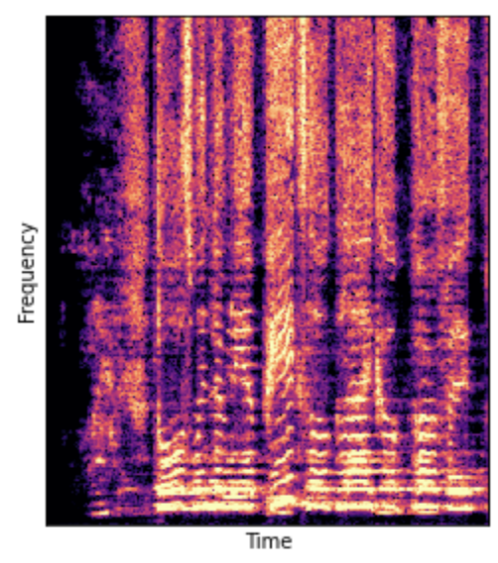
\includegraphics[width=0.6\textwidth]{research/dataset_preparation/PreprocessingSpecplot.png}
    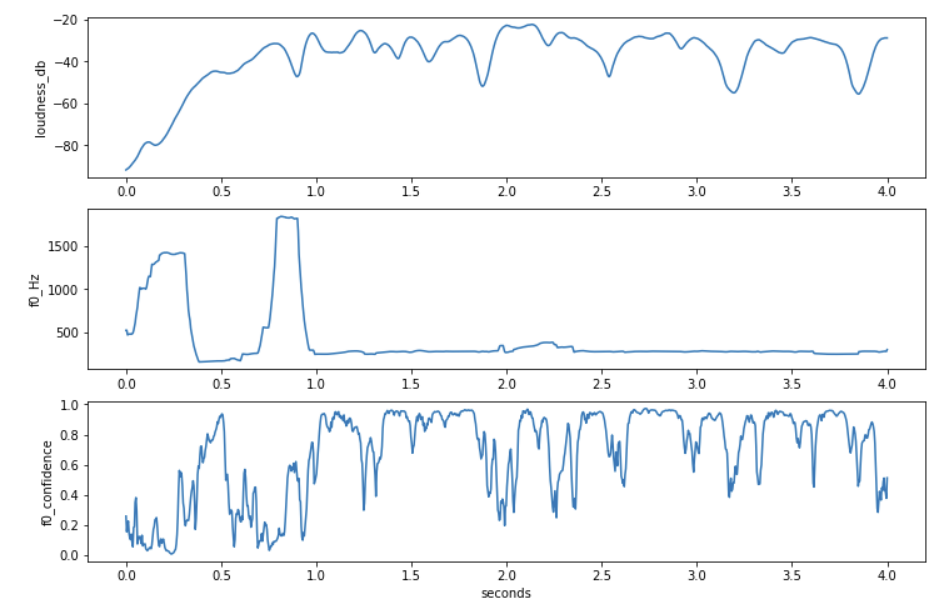
\includegraphics[width=0.8\textwidth]{research/dataset_preparation/PreprocessingFeatures.png}
    \caption{Dataset Pre-processing: Spectrogram plot of a random 4 second sample from one of the datasets and its accomanying F0, F0 Confidence and Amplitude characteristics over time throughout the sample}
\end{figure}

Pre-processing the datasets involved splitting the raw audio into smaller frames (samples), each 4 seconds long. The frame length was limited to 4 seconds to avoid capturing too much information in one spectrogram, which would make learning using the convolutional neural network difficult.

For each frame, F0 and confidence of F0 probability were inferred using CREPE\cite{CREPE}. Amplitude was computed statistically using the Librosa library\cite{LibrosaPip}. Latent Z information was available through the passing of the raw audio. The 4-second samples and accompanying features were then stored as TFRecord files.

Each of the two datasets was pre-processed on Google Colab notebooks; this process took approximately 40 minutes for each dataset using an NVIDIA Tesla V100 GPU.

Finally, a random 4-second clip was selected from each dataset to prove successful pre-processing. Its spectrogram was computed and plotted. Computed F0, F0 Confidence and Amplitude characteristics were also plotted for the selected clip. The underlying audio sample could also be played.

\section{Training}

A preprocessor was used that resampled the fundamental frequency and loudness, taking account the sample rate, frame rate, and number of timesteps. The number of timesteps was set at 1000 per 4 second clip, giving a spectral resoluiton of 4ms per timestep. This was deemed to be the best compromise between computational efficiency and accuracy.

An autoencoder encoder decoder setup was used. The encoder was based on Mfcc variant of a \acrfull{RNN}. The decoder was a RNN based decoder as described previously in \nameref{sec:singing_voice_synthesis}.

The model settings were kept the same as in \nameref{sec:singing_voice_synthesis} as they had already validated their hyperparameter selection. This included the use of100 sinusoidal harmonic components and 60 filter banks. This was done to limit model size to ensure it fitted on one GPU.

Each model was trained for 200,000 epochs, training time was approximately 2.9 epochs per second or 5.2 epochs per second depending on GPU used. Total training time was approxumately 20 horus per model.

\begin{figure}[!ht]
    \centering
    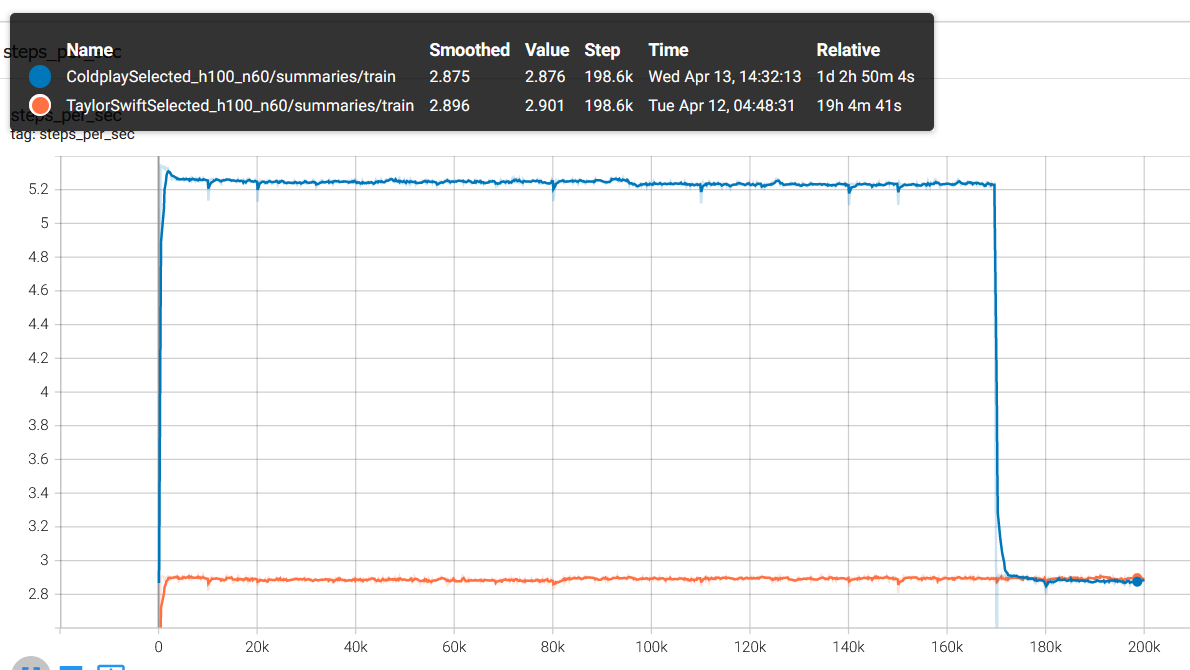
\includegraphics[width=0.6\textwidth]{research/training/StepsPerSecond.png}
    \caption{Training steps per second over the 200,000 training epochs}
\end{figure}

\begin{figure}[!ht]
    \centering
    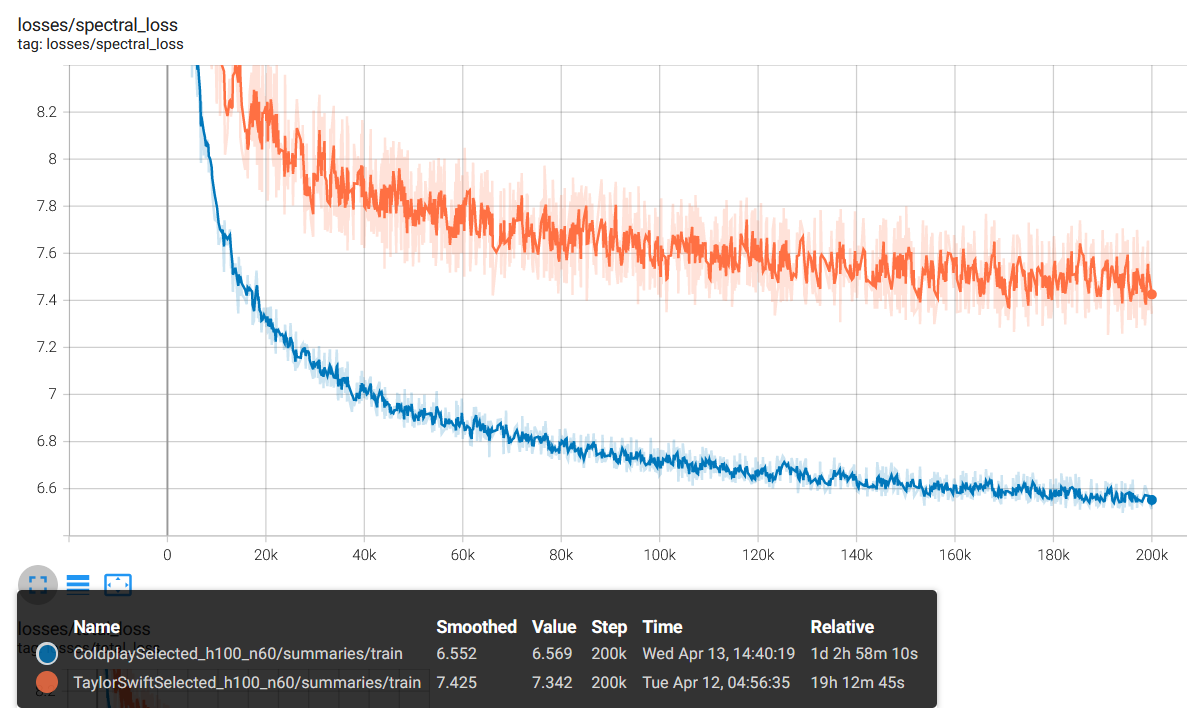
\includegraphics[width=0.8\textwidth]{research/training/TrainingSpectralLosses.png}
    \caption{Training Spectral Losses: Losses over the 200,000 epochs of training both models, using the spectral loss function defined in \nameref{sec:loss_measure}}
    \label{fig:training_spectral_losses}
\end{figure}

\nameref{fig:training_spectral_losses} shows the Coldplay losses being less than the Taylor Swift losses. This is due to the fact that the Coldplay Dataset having more frames that were pure silence, meaning that the Coldplay model fitted the silence frames more accurately.

